\documentclass[12pt,a4paper]{article}

% ─── Page Layout ───────────────────────────────────────────────────────────────
\usepackage[a4paper, margin=0.8in, headheight=14pt]{geometry}

% ─── Fonts (XeLaTeX) ───────────────────────────────────────────────────────────
\usepackage{fontspec}
\usepackage{unicode-math}
\setmainfont{TeX Gyre Pagella}
\setmonofont[Scale=0.88]{TeX Gyre Cursor}
\setmathfont{Latin Modern Math}

% ─── Packages ──────────────────────────────────────────────────────────────────
\usepackage{xcolor}
\usepackage{colortbl}
\usepackage{titlesec}
\usepackage{enumitem}
\usepackage{tabularx}
\usepackage{booktabs}
\usepackage{array}
\usepackage{amsmath}
\usepackage{tikz}
\usetikzlibrary{shapes.geometric, arrows.meta, positioning, calc, fit, decorations.pathreplacing, patterns}
\usepackage{tcolorbox}
\tcbuselibrary{skins, breakable}
\usepackage{hyperref}
\usepackage{fancyhdr}
\usepackage{graphicx}
\usepackage{microtype}
\hyphenpenalty=10000
\exhyphenpenalty=10000
\sloppy
\usepackage{caption}
\usepackage{setspace}
\usepackage{multirow}
\usepackage{tocloft}

% ─── Q&A helper ────────────────────────────────────────────────────────────────
\newcommand{\Q}[1]{\textbf{#1}\par\noindent\ignorespaces}

% ─── Colour Palette ────────────────────────────────────────────────────────────
\definecolor{myred}{RGB}{196,30,58}
\definecolor{mydark}{RGB}{30,30,50}
\definecolor{mygreen}{RGB}{14,120,80}
\definecolor{myteal}{RGB}{0,130,140}
\definecolor{myamber}{RGB}{180,100,0}
\definecolor{mypurple}{RGB}{100,30,160}
\definecolor{mygray}{RGB}{246,247,249}
\definecolor{mgframe}{RGB}{180,185,200}
\definecolor{watermark}{RGB}{145,150,170}
\definecolor{hdrred}{RGB}{250,232,235}
\definecolor{hdrgreen}{RGB}{220,244,233}
\definecolor{hdrteal}{RGB}{220,242,244}
\definecolor{hdramber}{RGB}{253,242,215}
\definecolor{hdrpurple}{RGB}{238,228,255}
\definecolor{hdrgray}{RGB}{238,240,245}
\definecolor{rowalt}{RGB}{250,251,253}

% ─── Section Formatting ────────────────────────────────────────────────────────
\titleformat{\section}
  {\large\bfseries\color{myred}}{\thesection.}{0.5em}{}
  [\vspace{1pt}{\color{myred}\rule{\linewidth}{0.8pt}}]
\titleformat{\subsection}
  {\normalsize\bfseries\color{myteal}}{\thesubsection}{0.5em}{}
\titlespacing*{\section}{0pt}{18pt}{7pt}
\titlespacing*{\subsection}{0pt}{11pt}{4pt}

% ─── Paragraph ─────────────────────────────────────────────────────────────────
\setlength{\parindent}{0pt}
\setlength{\parskip}{4pt}

% ─── TOC Styling ───────────────────────────────────────────────────────────────
\renewcommand{\cfttoctitlefont}{\large\bfseries\color{myred}}
\renewcommand{\cftaftertoctitle}{\par\noindent{\color{myred}\rule{\linewidth}{0.8pt}}}
\setlength{\cftbeforetoctitleskip}{0pt}
\setlength{\cftaftertoctitleskip}{6pt}
\renewcommand{\cftsecfont}{\normalsize\bfseries\color{mydark}}
\renewcommand{\cftsecpagefont}{\normalsize\bfseries\color{mydark}}
\renewcommand{\cftsecleader}{\cftdotfill{\cftdotsep}}
\setlength{\cftbeforesecskip}{7pt}
\renewcommand{\cftsubsecfont}{\small\color{mydark}}
\renewcommand{\cftsubsecpagefont}{\small\color{mydark}}
\setlength{\cftbeforesubsecskip}{3pt}
\setlength{\cftsubsecindent}{1.4em}

% ─── Table helpers ─────────────────────────────────────────────────────────────
\renewcommand{\arraystretch}{1.45}
\setlength{\tabcolsep}{6pt}
\arrayrulecolor{mydark}
\newcolumntype{B}[1]{>{\small\bfseries\raggedright\arraybackslash}m{#1}}
\newcolumntype{Y}{>{\small\raggedright\arraybackslash}X}
\renewcommand{\tabularxcolumn}[1]{m{#1}}

% ─── Header / Footer ───────────────────────────────────────────────────────────
\pagestyle{fancy}
\fancyhf{}
\fancyhead[L]{\small\color{myred}\textbf{EC402}\;\color{mydark}--- Analog Circuits}
\fancyhead[R]{\small\color{myteal}\textbf{Module 2 Notes}}
\fancyfoot[C]{\small\color{mydark}\thepage}
\fancyfoot[R]{\small\color{watermark}\textit{\copyright\ Biraj}}
\renewcommand{\headrulewidth}{0.5pt}
\renewcommand{\footrulewidth}{0.3pt}

% ─── Hyperref ──────────────────────────────────────────────────────────────────
\hypersetup{
  colorlinks=true, linkcolor=myteal, urlcolor=myteal,
  pdfauthor={Biraj Sarkar (CGEC)},
  pdftitle={EC402 --- Module 2 Notes: High Frequency Models, Frequency Response, Power Amplifiers and Feedback}
}

% ─── tcolorbox styles ──────────────────────────────────────────────────────────
\tcbset{
  tikzbox/.style={
    colback=mygray, colframe=mgframe, boxrule=0.6pt, arc=4pt,
    left=8pt, right=8pt, top=6pt, bottom=6pt,
    colbacktitle=mgframe, coltitle=mydark, fonttitle=\small\bfseries
  },
  defbox/.style={
    colback=hdrgreen, colframe=mygreen, boxrule=0.8pt, arc=4pt,
    left=9pt, right=9pt, top=6pt, bottom=6pt,
    colbacktitle=mygreen, coltitle=white, fonttitle=\small\bfseries
  },
  formulabox/.style={
    colback=hdrteal, colframe=myteal, boxrule=0.8pt, arc=4pt,
    left=9pt, right=9pt, top=7pt, bottom=7pt,
    colbacktitle=myteal, coltitle=white, fonttitle=\small\bfseries
  },
  examplebox/.style={
    colback=hdramber, colframe=myamber, boxrule=0.8pt, arc=4pt,
    left=9pt, right=9pt, top=6pt, bottom=6pt,
    colbacktitle=myamber, coltitle=white, fonttitle=\small\bfseries
  },
  masonbox/.style={
    colback=hdrpurple, colframe=mypurple, boxrule=0.8pt, arc=4pt,
    left=9pt, right=9pt, top=6pt, bottom=6pt,
    colbacktitle=mypurple, coltitle=white, fonttitle=\small\bfseries
  },
  exambox/.style={
    colback=hdrpurple, colframe=mypurple, boxrule=1pt, arc=5pt,
    left=10pt, right=10pt, top=8pt, bottom=8pt,
    colbacktitle=mypurple, coltitle=white, fonttitle=\bfseries,
    breakable, title after break={\textbf{Frequently Asked / Viva Questions (contd.)}}
  }
}
\tcbset{breakable}
\tcbset{after={\color{black}}}

% ─── TikZ styles ───────────────────────────────────────────────────────────────
\tikzset{
  block/.style={rectangle, draw=myteal, fill=hdrteal,
    text width=2.4cm, align=center, minimum height=0.95cm,
    font=\small, rounded corners=3pt, line width=0.7pt},
  redblock/.style={rectangle, draw=myred, fill=hdrred,
    text width=2.4cm, align=center, minimum height=0.95cm,
    font=\small, rounded corners=3pt, line width=0.7pt},
  sumjunc/.style={circle, draw=myamber, fill=hdramber,
    minimum size=0.62cm, font=\small, line width=0.8pt},
  arrow/.style={-Stealth, thick, color=mydark},
  redarrow/.style={-Stealth, thick, color=myred},
  line/.style={thick, color=mydark}
}

\begin{document}

% ─── Title Page ───────────────────────────────────────────────────────────────
\begin{center}
  {\LARGE\bfseries\color{myred} EC402 --- Analog Circuits}\\[5pt]
  {\normalsize\color{mydark} Semester IV \quad$\bullet$\quad 3L:0T:0P \quad$\bullet$\quad 3 Credits}\\[3pt]
  {\normalsize\color{myteal}\textbf{Module 2 Exam Notes: High Frequency Models, Frequency Response, Power Amplifiers and Feedback}}\\[3pt]
  {\small\color{mydark} CGEC \;$|$\; B.Tech ECE (2023--27) \;$|$\; \textit{Biraj Sarkar}}
\end{center}
\vspace{2pt}
\noindent{\color{myred}\rule{\linewidth}{1.5pt}}
\vspace{2pt}

\hypersetup{linkcolor=mydark}
\tableofcontents
\hypersetup{linkcolor=myteal}
\newpage

\section{High-Frequency Transistor Models and Miller's Theorem}

\begin{tcolorbox}[defbox, title={High-Frequency Hybrid-$\pi$ (Giacoletto) Model}]
At high frequencies ($f > 1\,\mathrm{MHz}$), internal parasitic junction capacitances cannot be neglected. The Giacoletto hybrid-$\pi$ model represents the intrinsic physical mechanism of a BJT:
\begin{itemize}[leftmargin=1.5em, itemsep=2pt]
  \item $r_{bb'}$: Base spreading resistance between external base terminal $B$ and internal active base $B'$ ($50$--$100\,\Omega$).
  \item $r_{b'e}$: Dynamic resistance of forward-biased emitter-base junction: $r_{b'e} = h_{fe} / g_m = \beta V_T / I_C$.
  \item $C_{b'e}$ (or $C_\pi$): Emitter diffusion capacitance ($C_d$) plus depletion capacitance ($C_{te}$): $C_{b'e} \approx \tau_F g_m$ ($20$--$100\,\mathrm{pF}$).
  \item $C_{b'c}$ (or $C_\mu$): Reverse-biased collector-base transition capacitance ($0.5$--$5\,\mathrm{pF}$). Provides feedback from output to input.
  \item $g_m v_{b'e}$: Voltage-controlled current source where $g_m = I_C/V_T$.
  \item $r_{ce}$: Early resistance representing base-width modulation: $r_{ce} = V_A / I_C$.
\end{itemize}
\end{tcolorbox}

\subsection{Transistor High-Frequency Figures of Merit: \texorpdfstring{$f_\beta$, $f_T$, and $f_{\max}$}{f_beta, f_T, and f_max}}
Consider a short-circuited collector load ($v_{ce} = 0$). The input current flows into $r_{b'e} \parallel C_{b'e} \parallel C_{b'c}$. The short-circuit current gain is:
\[
A_i(f) = \frac{I_c}{I_b} = \frac{g_m v_{b'e}}{v_{b'e}\left(\dfrac{1}{r_{b'e}} + j\omega (C_{b'e} + C_{b'c})\right)} = \frac{g_m r_{b'e}}{1 + j\omega r_{b'e}(C_{b'e} + C_{b'c})} = \frac{h_{fe}}{1 + j\left(\dfrac{f}{f_\beta}\right)}.
\]

\begin{tcolorbox}[formulabox, title={Cutoff and Unity-Gain Frequencies}]
\begin{enumerate}[leftmargin=1.5em, itemsep=2pt]
  \item \textbf{Beta Cutoff Frequency ($f_\beta$)}: Frequency at which common-emitter current gain drops by $3\,\mathrm{dB}$ ($0.707 h_{fe}$):
  \[
  f_\beta = \frac{1}{2\pi r_{b'e}(C_{b'e} + C_{b'c})}.
  \]
  \item \textbf{Unity-Gain Frequency ($f_T$)}: Frequency at which short-circuit current gain drops to unity ($|A_i(f_T)| = 1$):
  \[
  f_T \approx h_{fe} f_\beta = \frac{g_m}{2\pi (C_{b'e} + C_{b'c})}.
  \]
  \item \textbf{Maximum Oscillation Frequency ($f_{\max}$)}: Frequency at which unilateral power gain drops to unity:
  \[
  f_{\max} = \sqrt{\frac{f_T}{8\pi r_{bb'} C_{b'c}}}.
  \]
\end{enumerate}
\end{tcolorbox}

\subsection{Miller's Theorem and the Miller Effect}
\begin{tcolorbox}[defbox, title={Miller's Theorem}]
Any feedback impedance $Z$ connected between an input node $1$ and an inverting output node $2$ with voltage gain $A_v = V_2/V_1$ can be replaced by two uncoupled grounded impedances:
\[
Z_{M1} = \frac{Z}{1 - A_v}\quad\text{(Input Side)},\qquad
Z_{M2} = \frac{Z}{1 - 1/A_v} \approx Z\quad\text{(Output Side for } |A_v| \gg 1\text{)}.
\]
\end{tcolorbox}

For a feedback capacitance $C_f = C_{b'c}$ across an inverting amplifier ($A_v = -|A_v|$):
\[
\frac{1}{j\omega C_{M1}} = \frac{1}{j\omega C_f(1 + |A_v|)} \implies C_{M1} = C_f(1 + |A_v|).
\]
\textbf{The Miller Effect}: The bridging collector-base capacitance $C_{b'c}$ appears at the input magnified by $(1 + |A_v|)$. Because inverting amplifiers typically have high voltage gain ($|A_v| \sim 100$--$300$), $C_{M1}$ becomes huge ($100$--$500\,\mathrm{pF}$), severely reducing the upper $3\,\mathrm{dB}$ cutoff frequency $f_H$.

\section{Frequency Response of Amplifiers and the Cascode Configuration}

\subsection{Bode Response and Cutoff Frequencies}
The frequency response of an $RC$-coupled amplifier is divided into three distinct operational regions:
\begin{enumerate}[leftmargin=1.5em, itemsep=2pt]
  \item \textbf{Low-Frequency Band ($f < f_L$)}: Voltage gain rolls off at $+20\,\mathrm{dB/decade}$ due to the rising reactances of input coupling capacitor $C_{C1}$, output coupling capacitor $C_{C2}$, and emitter bypass capacitor $C_E$:
  \[
  f_L \approx \frac{1}{2\pi R_{th,C1} C_{C1}} + \frac{1}{2\pi R_{th,C2} C_{C2}} + \frac{1}{2\pi R_{th,E} C_E}.
  \]
  \item \textbf{Mid-Frequency Band ($f_L \le f \le f_H$)}: Coupling and bypass capacitors act as perfect $ac$ short circuits; parasitic capacitances act as open circuits. Voltage gain is flat ($A_{vm}$).
  \item \textbf{High-Frequency Band ($f > f_H$)}: Gain rolls off at $-20\,\mathrm{dB/decade}$ due to parasitic junction capacitances ($C_{b'e}$) and Miller-multiplied input capacitance ($C_{Mi}$):
  \[
  f_H \approx \frac{1}{2\pi R_{\rm in}' \left[C_{b'e} + C_{b'c}(1 + g_m R_L')\right]}.
  \]
\end{enumerate}

\begin{tcolorbox}[formulabox, title={Bandwidth and Multistage Shrinkage Factors}]
\begin{enumerate}[leftmargin=1.5em, itemsep=2pt]
  \item \textbf{Bandwidth}: $\mathrm{BW} = f_H - f_L \approx f_H$ (since $f_H \gg f_L$).
  \item \textbf{Gain-Bandwidth Product (GBW)}: $\mathrm{GBW} = |A_{vm}| \times \mathrm{BW} = \mathrm{constant}$.
  \item \textbf{Multistage Cascading Shrinkage}: For $n$ identical cascaded stages with lower cutoff $f_L$ and upper cutoff $f_H$:
  \[
  f_{L(n)} = \frac{f_L}{\sqrt{2^{1/n} - 1}},\qquad
  f_{H(n)} = f_H \sqrt{2^{1/n} - 1}.
  \]
  Cascading increases lower cutoff $f_{L(n)}$ and decreases upper cutoff $f_{H(n)}$, drastically reducing net bandwidth.
\end{enumerate}
\end{tcolorbox}

\subsection{The Cascode Amplifier (CE--CB Configuration)}
\begin{tcolorbox}[defbox, title={Cascode Topology and Miller Effect Elimination}]
A \textbf{Cascode Amplifier} consists of a Common-Emitter (CE) input stage $Q_1$ driving a Common-Base (CB) output stage $Q_2$ in series:
\begin{itemize}[leftmargin=1.5em, itemsep=2pt]
  \item $Q_1$ provides high input resistance $R_{in} = r_{\pi 1}$.
  \item The load seen by the collector of $Q_1$ is the low input resistance of $Q_2$: $R_{L1} = R_{in2} \approx r_{e2} = 1/g_{m2}$.
  \item Voltage gain of the first stage is only $A_{v1} \approx -g_{m1} R_{in2} = -g_{m1}(1/g_{m2}) \approx -1$.
  \item The Miller input capacitance of $Q_1$ becomes:
  \[
  C_{M1} = C_{b'c1}(1 + |A_{v1}|) \approx 2 C_{b'c1}.
  \]
  \item The CB stage $Q_2$ provides the full voltage gain $A_{v2} = +g_{m2} R_C$, but CB exhibits zero Miller effect because its base is $ac$ grounded.
  \item \textbf{Result}: Overall voltage gain is $A_v = A_{v1} A_{v2} \approx -g_{m1} R_C$ (identical to a single CE), while the high-frequency cutoff $f_H$ increases by a factor of $50$--$100$.
\end{itemize}
\end{tcolorbox}

\begin{tcolorbox}[tikzbox, unbreakable, title={Cascode (CE--CB) Circuit Architecture}]
\centering
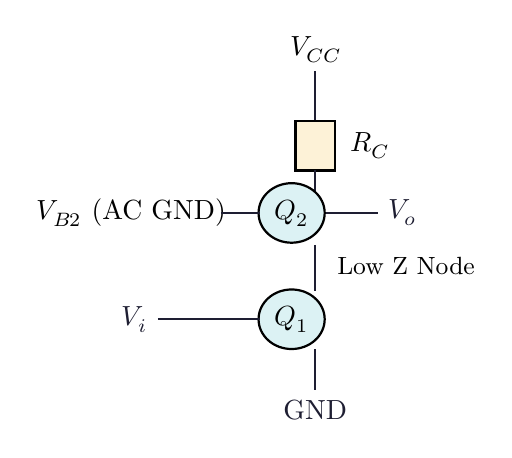
\begin{tikzpicture}[x=1cm,y=0.9cm]
  \node at (2,4.8) {$V_{CC}$};
  \draw[line] (2,4.5)--(2,3.8);
  \draw[thick,fill=hdramber] (1.75,3.1) rectangle (2.25,3.8);
  \node[right=2pt] at (2.25,3.45) {$R_C$};
  \draw[line] (2,3.1)--(2,2.5);
  \draw[line] (2,2.5)--(2.8,2.5) node[right] {$V_o$};

  % Q2 (CB)
  \draw[thick,fill=hdrteal] (1.7,2.5) circle (0.42);
  \node at (1.7,2.5) {$Q_2$};
  \node[left=6pt] at (1.2,2.5) {$V_{B2}$ (AC GND)};
  \draw[line] (0.8,2.5)--(1.3,2.5);

  \draw[line] (2,2.05)--(2,1.4);
  \node[right=3pt] at (2.05,1.75) {\small Low Z Node};

  % Q1 (CE)
  \draw[thick,fill=hdrteal] (1.7,1.0) circle (0.42);
  \node at (1.7,1.0) {$Q_1$};
  \draw[line] (0,1.0)--(1.3,1.0) node[pos=0,left] {$V_i$};
  \draw[line] (2,0.58)--(2,0) node[below] {GND};
\end{tikzpicture}\par
\small Input stage $Q_1$ sees load $R_{in2} \approx 1/g_m \approx 26\,\Omega$, keeping $|A_{v1}| \approx 1$ and suppressing Miller multiplication.
\end{tcolorbox}

\section{Power Amplifiers (Large-Signal Classification)}

\begin{tcolorbox}[defbox, title={Classification of Power Amplifiers by Conduction Angle}]
Power amplifiers are designed to deliver maximum $ac$ power to a low-impedance load (e.g., $4\,\Omega$--$8\,\Omega$ loudspeaker) with minimum harmonic distortion and maximum collector conversion efficiency $\eta = P_{ac} / P_{dc}$.
\end{tcolorbox}

\par\vspace{6pt}\noindent
\begin{tabularx}{\linewidth}{|B{2.2cm}|B{2.6cm}|B{2.7cm}|Y|}
\hline
\textbf{Class} & \textbf{Conduction Angle ($\theta$)} & \textbf{Max Efficiency ($\eta$)} & \textbf{Distortion \& Applications} \\
\hline
\textbf{Class A} & $360^\circ$ (Full cycle) & $25\%$ (Series-fed)\newline $50\%$\newline (Transformer) & Lowest distortion; high quiescent dissipation; audio preamps. \\
\hline
\textbf{Class B} & $180^\circ$ (Half cycle) & $\frac{\pi}{4} \approx 78.5\%$ & Push-pull topology; suffers from \textbf{crossover distortion}. \\
\hline
\textbf{Class AB}& $180^\circ < \theta < 360^\circ$ & $50\%$ to $78.5\%$ & Slight forward bias eliminates crossover distortion; standard audio output stage. \\
\hline
\textbf{Class C} & $\theta < 180^\circ$ ($\sim 120^\circ$) & $> 85\%$ & Extreme non-linearity; tuned LC tank extracts carrier; RF transmitters. \\
\hline
\textbf{Class D} & Switching (PWM) & $\approx 95\%$--$98\%$ & Transistors act as on/off switches; negligible dissipation; modern compact audio/subwoofers. \\
\hline
\end{tabularx}
\par\vspace{12pt}

\subsection{Class B and Class AB Push-Pull Operation}
In a Class B push-pull amplifier, two complementary transistors ($NPN$ and $PNP$) conduct alternately:
\[
\begin{aligned}
P_{dc} &= V_{CC} I_{dc} = V_{CC} \left(\frac{2I_m}{\pi}\right) = \frac{2V_{CC}V_m}{\pi R_L},\\
P_{ac} &= \frac{V_m^2}{2R_L},\\
\eta &= \frac{P_{ac}}{P_{dc}} = \frac{V_m^2 / (2R_L)}{2V_{CC}V_m / (\pi R_L)} = \frac{\pi}{4}\left(\frac{V_m}{V_{CC}}\right).
\end{aligned}
\]
At maximum unclipped swing ($V_m = V_{CC}$), efficiency reaches $\eta_{\max} = \pi/4 \approx 78.5\%$.
\begin{itemize}[leftmargin=1.5em, itemsep=2pt]
  \item \textbf{Crossover Distortion}: Neither transistor conducts when the input voltage is within $\pm 0.7\,\mathrm{V}$ of zero (below the cut-in voltage $V_\gamma$). This creates a dead band in the output waveform.
  \item \textbf{Class AB Remedy}: Biasing diodes or a $V_{BE}$-multiplier circuit provide a small quiescent forward bias voltage ($V_{bias} \approx 2 V_\gamma \approx 1.4\,\mathrm{V}$), maintaining a trickle quiescent current ($I_{CQ}$) that eliminates crossover distortion.
\end{itemize}

\section{Feedback Amplifiers: Topologies and Systematic Analysis}

\begin{tcolorbox}[defbox, title={Feedback Principle and Closed-Loop Gain}]
Negative feedback samples the output signal $X_o$ and feeds back a fraction $X_f = \beta X_o$ in phase opposition to the input signal $X_s$. The error signal applied to the basic amplifier is $X_i = X_s - X_f$.
\[
A_f = \frac{X_o}{X_s} = \frac{A X_i}{X_i + \beta A X_i} = \frac{A}{1 + A\beta}.
\]
Here $A$ is open-loop gain, $\beta$ is feedback factor, $A\beta$ is loop gain, and $(1+A\beta)$ is the \textbf{desensitivity / feedback factor}.
\end{tcolorbox}

\subsection{The Four Basic Feedback Topologies}
Depending on whether the output voltage or current is sampled, and whether the feedback signal is mixed in series (voltage subtraction) or shunt (current subtraction):

\begin{enumerate}[leftmargin=1.5em, itemsep=3pt]
  \item \textbf{Voltage-Series (Series-Shunt) Feedback}: Samples output voltage, mixes feedback voltage in series at input:
  \[
  R_{if} = R_i (1 + A\beta),\qquad R_{of} = \frac{R_o}{1 + A\beta}.
  \]
  \textit{Ideal for Voltage Amplifiers} ($R_{if} \to \infty, R_{of} \to 0$). Example: Non-inverting Op-Amp, Emitter Follower.
  \item \textbf{Current-Series (Series-Series) Feedback}: Samples output current, mixes feedback voltage in series:
  \[
  R_{if} = R_i (1 + A\beta),\qquad R_{of} = R_o (1 + A\beta).
  \]
  \textit{Ideal for Transconductance Amplifiers} ($R_{if} \to \infty, R_{of} \to \infty$). Example: CE amplifier with unbypassed emitter resistor $R_E$.
  \item \textbf{Voltage-Shunt (Shunt-Shunt) Feedback}: Samples output voltage, mixes feedback current in shunt:
  \[
  R_{if} = \frac{R_i}{1 + A\beta},\qquad R_{of} = \frac{R_o}{1 + A\beta}.
  \]
  \textit{Ideal for Transresistance Amplifiers} ($R_{if} \to 0, R_{of} \to 0$). Example: Collector-base feedback resistor amplifier, Inverting Op-Amp.
  \item \textbf{Current-Shunt (Shunt-Series) Feedback}: Samples output current, mixes feedback current in shunt:
  \[
  R_{if} = \frac{R_i}{1 + A\beta},\qquad R_{of} = R_o (1 + A\beta).
  \]
  \textit{Ideal for Current Amplifiers} ($R_{if} \to 0, R_{of} \to \infty$). Example: Two-stage BJT current amplifier with emitter-to-base feedback.
\end{enumerate}

\subsection{Effects of Negative Feedback on Amplifier Performance}
\begin{tcolorbox}[formulabox, title={Quantitative Benefits of Negative Feedback}]
\begin{enumerate}[leftmargin=1.5em, itemsep=2pt]
  \item \textbf{Gain Desensitization}:
  Differentiating $A_f = A/(1+A\beta)$:
  \[
  \frac{dA_f}{A_f} = \frac{1}{1 + A\beta}\left(\frac{dA}{A}\right).
  \]
  Gain stability increases by the factor $(1+A\beta)$.
  \item \textbf{Bandwidth Extension}:
  Upper cutoff increases and lower cutoff decreases:
  \[
  f_{Hf} = f_H (1 + A\beta),\qquad f_{Lf} = \frac{f_L}{1 + A\beta},\qquad \mathrm{BW}_f \approx \mathrm{BW}(1 + A\beta).
  \]
  \item \textbf{Non-Linear Harmonic Distortion Reduction}:
  Harmonic distortion generated within the amplifier is suppressed:
  \[
  D_f = \frac{D}{1 + A\beta}.
  \]
  \item \textbf{Noise Reduction}: Noise generated within the feedback loop is reduced by $(1+A\beta)$. (Noise present at the signal source is amplified equally).
\end{enumerate}
\end{tcolorbox}

\begin{tcolorbox}[examplebox, title={Gain Stabilization and Bandwidth Expansion Calculation}]
An open-loop amplifier has $A = 1000 \pm 100$ ($10\%$ variation), $f_L = 50\,\mathrm{Hz}$, and $f_H = 20\,\mathrm{kHz}$. Design negative feedback with $\beta = 0.049$.
\[
\begin{aligned}
\text{Desensitivity factor:}\quad 1 + A\beta &= 1 + 1000(0.049) = 1 + 49 = 50,\\
\text{Closed-loop gain:}\quad A_f &= \frac{A}{1 + A\beta} = \frac{1000}{50} = 20,\\
\text{Fractional gain variation:}\quad \frac{dA_f}{A_f} &= \frac{1}{50}\left(\frac{dA}{A}\right) = \frac{10\%}{50} = 0.2\%,\\
\text{New bandwidth:}\quad f_{Hf} &= 20\,\mathrm{kHz} \times 50 = 1000\,\mathrm{kHz} = 1\,\mathrm{MHz},\\
f_{Lf} &= 50\,\mathrm{Hz} / 50 = 1\,\mathrm{Hz}.
\end{aligned}
\]
Negative feedback stabilizes gain to within $0.2\%$ and expands bandwidth from $20\,\mathrm{kHz}$ to $1\,\mathrm{MHz}$.
\end{tcolorbox}

\newpage

% ─── Quick Revision Page ───────────────────────────────────────────────────────
\begin{center}
  {\large\bfseries\color{myred} Quick Revision --- Module 2}\\[3pt]
  {\small\color{mydark} Frequency Response, Power Amplifiers and Feedback $|$ EC402}
\end{center}
\noindent{\color{myred}\rule{\linewidth}{1.2pt}}
\vspace{4pt}

\begin{tcolorbox}[formulabox, title={Key Formulas at a Glance}]
\small
\renewcommand{\arraystretch}{1.35}
\setlength{\tabcolsep}{5pt}
\noindent\begin{tabularx}{\linewidth}{B{4.1cm}Y}
Beta Cutoff Frequency ($f_\beta$) & $f_\beta = \frac{1}{2\pi r_{b'e}(C_{b'e}+C_{b'c})} = \frac{1}{2\pi r_\pi (C_\pi + C_\mu)}$ \\[3pt]
Unity-Gain Frequency ($f_T$) & $f_T = h_{fe} f_\beta = \frac{g_m}{2\pi (C_{b'e}+C_{b'c})}$ \\[3pt]
Miller Input Capacitance & $C_{Mi} = C_f(1 + |A_v|)$ \newline $C_{Mo} = C_f(1 + 1/|A_v|) \approx C_f$ \\[3pt]
Multistage Bandwidth Shrink & $f_{H(n)} = f_H \sqrt{2^{1/n}-1}$ \newline $f_{L(n)} = f_L / \sqrt{2^{1/n}-1}$ \\[3pt]
Cascode Miller Capacitance & $C_{M1} = C_{b'c1}(1 + |-1|) = 2C_{b'c1}$ (virtually no Miller multiplication) \\[3pt]
Class B Efficiency ($\eta$) & $\eta = \frac{\pi}{4}\left(\frac{V_m}{V_{CC}}\right)$ \newline $\eta_{\max} = \frac{\pi}{4} \approx 78.5\%$ \\[3pt]
Closed-Loop Feedback Gain & $A_f = \frac{A}{1+A\beta}$ \newline Desensitivity factor $= (1+A\beta)$ \\[3pt]
Feedback Input Resistance & $R_{if} = R_i(1+A\beta)$ (Series) \newline $R_{if} = R_i/(1+A\beta)$ (Shunt) \\[3pt]
Feedback Output Resistance & $R_{of} = R_o/(1+A\beta)$ (Voltage) \newline $R_{of} = R_o(1+A\beta)$ (Current) \\[3pt]
Distortion \& Noise Reduction& $D_f = \frac{D}{1+A\beta}$ \newline $\mathrm{BW}_f = \mathrm{BW}(1+A\beta)$
\end{tabularx}\par
\end{tcolorbox}

\begin{tcolorbox}[defbox, title={One-Line Definitions}, title after break={One-Line Definitions (contd.)}]
\small
\begin{itemize}[leftmargin=1.5em, topsep=2pt, itemsep=4pt]
  \item \textbf{Beta Cutoff Frequency ($f_\beta$)}: The frequency at which the common-emitter short-circuit current gain drops by $3\,\mathrm{dB}$ ($0.707$) from its low-frequency value $h_{fe}$.
  \item \textbf{Unity-Gain Frequency ($f_T$)}: The frequency at which the short-circuit forward current gain of a BJT drops to unity ($0\,\mathrm{dB}$).
  \item \textbf{Miller Effect}: The dramatic increase in equivalent input capacitance of an inverting amplifier stage caused by feedback capacitance multiplication by $(1 + |A_v|)$.
  \item \textbf{Cascode Amplifier}: A two-stage compound configuration consisting of a common-emitter stage feeding a common-base stage that suppresses the Miller effect.
  \item \textbf{Cross-Over Distortion}: The dead-band zero-crossing distortion in Class B push-pull amplifiers occurring because input voltage falls below the diode cut-in threshold ($V_\gamma \approx 0.7\,\mathrm{V}$).
  \item \textbf{Conduction Angle}: The total portion of an input sinusoidal cycle (in degrees or radians) during which the active output device conducts current.
  \item \textbf{Desensitivity}: The factor $(1+A\beta)$ by which fractional variations in open-loop gain are suppressed under negative feedback: $dA_f/A_f = (1/(1+A\beta))(dA/A)$.
  \item \textbf{Voltage-Series Feedback}: A feedback topology that samples output voltage and feeds back a proportional voltage in series opposition, raising input impedance and lowering output impedance.
\end{itemize}
\end{tcolorbox}

\begin{tcolorbox}[exambox, title={Frequently Asked / Viva Questions}]
\begin{enumerate}[topsep=0pt, label=\textbf{Q\arabic*.}, itemsep=5pt]
  \item \Q{What is the physical origin of $C_{b'e}$ and $C_{b'c}$ in the Giacoletto model?}
  $C_{b'e}$ is dominated by the forward-bias emitter diffusion capacitance $C_d$ (caused by minority carrier storage in the base); $C_{b'c}$ is the transition/depletion capacitance of the reverse-biased collector-base junction.

  \item \Q{Why does a Common Emitter amplifier have a much lower high-frequency cutoff than a Common Base amplifier?}
  Because the CE amplifier has high inverting voltage gain, triggering the Miller effect which multiplies $C_{b'c}$ by $(1+|A_v|)$ to create a huge shunt input capacitance; in CB, the base is grounded, completely decoupling input from output.

  \item \Q{How does the Cascode configuration eliminate the Miller effect without sacrificing voltage gain?}
  The input CE transistor drives the low input impedance of the CB stage ($1/g_m$), holding the CE stage voltage gain at $A_{v1} \approx -1$ so its Miller multiplier is only $(1+1)=2$; the CB stage then provides the full voltage gain without any Miller multiplication.

  \item \Q{Why is the maximum theoretical efficiency of a Class B amplifier $78.5\%$ while Class A is only $25\%$?}
  In Class A, DC current flows for the full $360^\circ$ even with zero input signal, causing massive standby dissipation; Class B draws current only for $180^\circ$ in proportion to the signal, with zero standby dissipation under quiescent conditions.

  \item \Q{How is cross-over distortion completely eliminated in audio power amplifiers?}
  By operating in Class AB: placing two forward-biased diodes (or a $V_{BE}$-multiplier circuit) between the bases of the complementary transistors, maintaining a small quiescent trickle bias ($V_{BB} \approx 1.4\,\mathrm{V}$).

  \item \Q{What are the four feedback topologies and their effect on terminal impedances?}
  Voltage-series: $R_i \uparrow, R_o \downarrow$; Current-series: $R_i \uparrow, R_o \uparrow$; Voltage-shunt: $R_i \downarrow, R_o \downarrow$; Current-shunt: $R_i \downarrow, R_o \uparrow$.

  \item \Q{Prove that negative feedback expands amplifier bandwidth.}
  With feedback, $f_{Hf} = f_H(1+A\beta)$ and $f_{Lf} = f_L/(1+A\beta)$. Thus, upper cutoff increases and lower cutoff decreases by the same factor $(1+A\beta)$, expanding total bandwidth while maintaining a constant gain-bandwidth product.

  \item \Q{Why does negative feedback reduce non-linear harmonic distortion?}
  Non-linearities generated within the amplifier produce distortion harmonics that are sampled and fed back out-of-phase to the input, canceling a fraction $(1+A\beta)$ of the internal distortion: $D_f = D/(1+A\beta)$.

  \item \Q{Does negative feedback reduce noise present at the input signal source?}
  No. Negative feedback attenuates internal noise generated inside the amplifier loop by $(1+A\beta)$, but input noise entering with the signal is amplified by the exact same closed-loop gain $A_f$, leaving the input SNR unchanged.

  \item \Q{What happens to the overall bandwidth when $n$ identical amplifier stages are cascaded?}
  Overall bandwidth shrinks significantly: $f_{H(n)} = f_H \sqrt{2^{1/n}-1}$ and $f_{L(n)} = f_L / \sqrt{2^{1/n}-1}$. For two stages ($n=2$), $f_{H(2)} \approx 0.64 f_H$ ($36\%$ bandwidth reduction).
\end{enumerate}
\end{tcolorbox}

\begin{tcolorbox}[tikzbox, title={Summary Comparison of the Four Feedback Topologies}]
\renewcommand{\arraystretch}{1.25}
\setlength{\tabcolsep}{5pt}
\noindent\begin{tabularx}{\linewidth}{|B{3.2cm}|B{2.6cm}|B{2.2cm}|B{2.2cm}|Y|}
\hline
\textbf{Topology} & \textbf{Sampled Quantity} & \textbf{Mixed Quantity} & \textbf{Input / Output Z} & \textbf{Ideal Amplifier Type} \\
\hline
\textbf{Voltage-Series} & Output Voltage ($V_o$) & Voltage in Series ($V_f$) & $R_{in}\uparrow$ / $R_{out}\downarrow$ & Voltage Amplifier ($A_v$) \\
\hline
\textbf{Current-Series} & Output Current ($I_o$) & Voltage in Series ($V_f$) & $R_{in}\uparrow$ / $R_{out}\uparrow$ & Transconductance ($G_m$) \\
\hline
\textbf{Voltage-Shunt}  & Output Voltage ($V_o$) & Current in Shunt ($I_f$) & $R_{in}\downarrow$ / $R_{out}\downarrow$ & Transresistance ($R_m$) \\
\hline
\textbf{Current-Shunt}  & Output Current ($I_o$) & Current in Shunt ($I_f$) & $R_{in}\downarrow$ / $R_{out}\uparrow$ & Current Amplifier ($A_i$) \\
\hline
\end{tabularx}\par
\end{tcolorbox}

\end{document}
